% arara: pdflatex: { shell: yes }
\documentclass[twoside]{article}
\usepackage[utf8]{inputenc}
\usepackage[english]{babel}
\usepackage{amsmath, amssymb, amsthm}
\usepackage{hyperref}
\usepackage{ragged2e}
\usepackage{graphicx}
\usepackage{float}
\usepackage{fancyhdr}
\usepackage{geometry}
\usepackage{multicol}
\usepackage{url}

% Suppress underfull and overfull warnings
\tolerance=1000
\emergencystretch=10pt

\setlength{\headheight}{15.2pt}
\geometry{paperwidth=8.5in, paperheight=11.0in, top=1.0in, bottom=1.0in, left=1.0in, right=1.0in}

\pagestyle{fancyplain}
\fancyhead[LO]{Project Report}
\fancyhead[CO]{}
\fancyhead[RO]{P25-LIS3082-2}
\fancyfoot[LO]{\thepage}
\fancyfoot[CO]{Artificial Intelligence, UDLAP}
\fancyfoot[RO]{}

\begin{document}

\fancypagestyle{plain}{
    \renewcommand{\headrulewidth}{1pt}
    \renewcommand{\footrulewidth}{1pt}
}

\title{Project Report}
\author{\small{Erick Gonzalez Parada ID: 178145}\\
\small{Paulo Stefano Westermann ID: 185573}}
\date{\today}
\maketitle

\begin{abstract}
A modular neural network was developed to predict diverse mathematical properties of numbers, providing instant, explainable results for data science and mathematics. 
\end{abstract}


\begin{multicols}{2}

\section{Objectives}
\begin{itemize}
    \item Design and implement a NumPy-based neural network to predict mathematical properties of numbers.
    \item Provide instant access to number properties for mathematicians and data scientists.
    \item Evaluate model performance using precision, recall, F1-score, and visualizations.
    \item Demonstrate the utility of the tool for Zero Knowledge Proof and explainable AI.
\end{itemize}

\section{Problematic}
The lack of ``Zero Knowledge Proof'' in data science and artificial intelligence fields presents a challenge for transparency and trust. By providing a tool that instantly reveals the mathematical properties of any number, this project aids mathematicians and data scientists in verifying and understanding number characteristics, thus promoting explainability and trustworthiness in computational mathematics.

\section{Theoretical Background}
Zero Knowledge Proof (ZKP) is a cryptographic concept allowing one party to prove to another that a statement is true, without revealing any information beyond the validity of the statement \cite{zeroknowledgeproof}. While ZKP is not yet widely implemented in data science, the ability to instantly verify number properties aligns with its goals of transparency and trust.

Neural networks, inspired by biological neurons, are widely used in artificial intelligence for pattern recognition and classification tasks \cite{neuralnetwork}. In this project, a modular NumPy-based neural network is trained to classify numbers according to mathematical properties such as primality, being a perfect number, Fibonacci sequence membership \cite{fibonnacisequence}, palindrome, Armstrong, Harshad, square-free, abundant, deficient, happy, triangular, and Catalan numbers.

Model performance is assessed using standard classification metrics: precision, recall, and F1-score, along with confusion matrices, ROC and PR curves, and learning curves. These metrics provide a comprehensive understanding of the model's strengths and weaknesses in classifying rare and common properties.

\section{Methodology}
A modular neural network architecture was implemented in Python using NumPy, with one neuron per property. Training data for each property was generated using mathematical definitions. For each property, the network was trained and tested on a large range of integers, and the following metrics were computed: accuracy, precision, recall, F1-score. Visualizations include bar charts of metrics, confusion matrices, ROC and PR curves, and learning curves. All results are automatically saved for further analysis.

\section{Results}
% Confusion matrix plots for each property
\begin{figure}[H]
    \centering
    \includegraphics[width=0.45\textwidth]{plots/odd_even_confusion.png}
    \caption{Odd/Even Confusion Matrix}
\end{figure}
\begin{figure}[H]
    \centering
    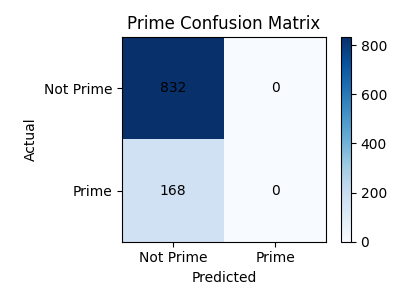
\includegraphics[width=0.45\textwidth]{plots/prime_confusion.png}
    \caption{Prime Confusion Matrix}
\end{figure}
\begin{figure}[H]
    \centering
    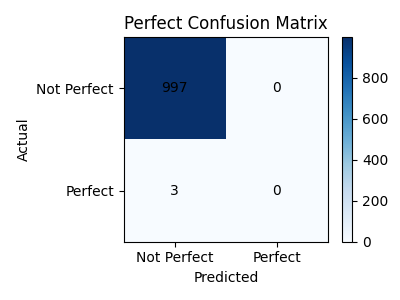
\includegraphics[width=0.45\textwidth]{plots/perfect_confusion.png}
    \caption{Perfect Confusion Matrix}
\end{figure}
\begin{figure}[H]
    \centering
    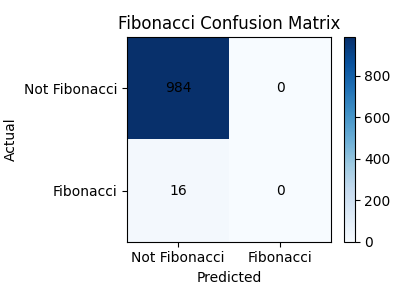
\includegraphics[width=0.45\textwidth]{plots/fibonacci_confusion.png}
    \caption{Fibonacci Confusion Matrix}
\end{figure}
\begin{figure}[H]
    \centering
    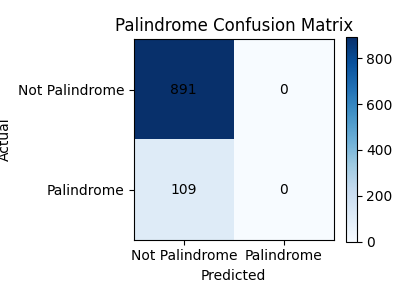
\includegraphics[width=0.45\textwidth]{plots/palindrome_confusion.png}
    \caption{Palindrome Confusion Matrix}
\end{figure}
\begin{figure}[H]
    \centering
    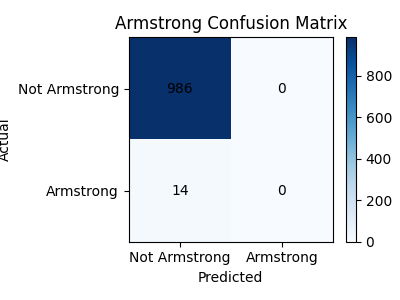
\includegraphics[width=0.45\textwidth]{plots/armstrong_confusion.png}
    \caption{Armstrong Confusion Matrix}
\end{figure}
\begin{figure}[H]
    \centering
    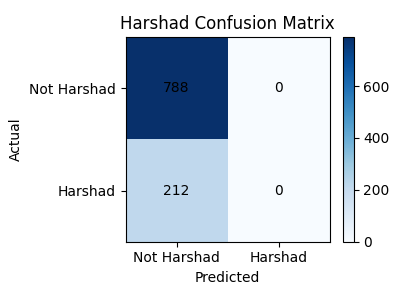
\includegraphics[width=0.45\textwidth]{plots/harshad_confusion.png}
    \caption{Harshad Confusion Matrix}
\end{figure}
\begin{figure}[H]
    \centering
    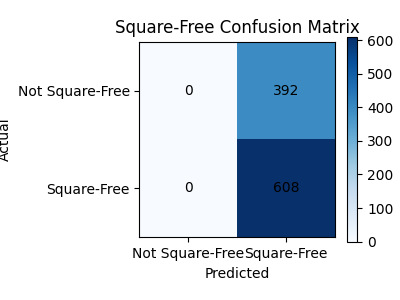
\includegraphics[width=0.45\textwidth]{plots/square-free_confusion.png}
    \caption{Square-Free Confusion Matrix}
\end{figure}
\begin{figure}[H]
    \centering
    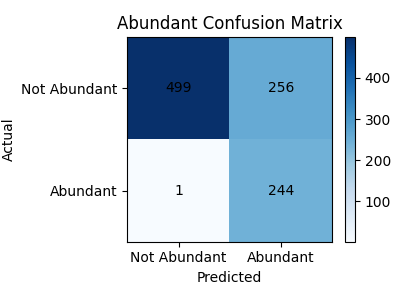
\includegraphics[width=0.45\textwidth]{plots/abundant_confusion.png}
    \caption{Abundant Confusion Matrix}
\end{figure}
\begin{figure}[H]
    \centering
    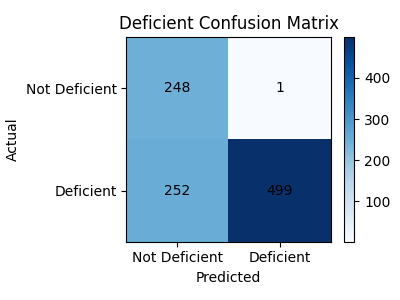
\includegraphics[width=0.45\textwidth]{plots/deficient_confusion.png}
    \caption{Deficient Confusion Matrix}
\end{figure}
\begin{figure}[H]
    \centering
    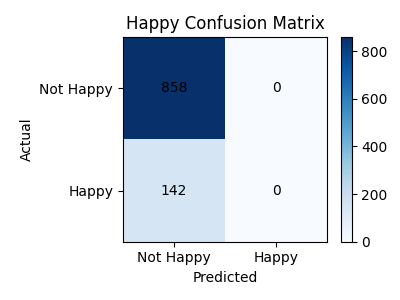
\includegraphics[width=0.45\textwidth]{plots/happy_confusion.png}
    \caption{Happy Confusion Matrix}
\end{figure}
\begin{figure}[H]
    \centering
    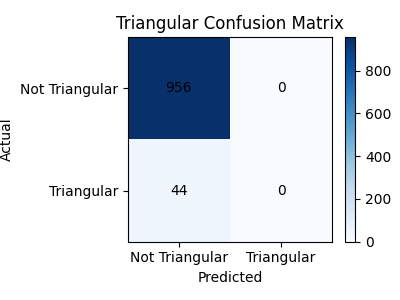
\includegraphics[width=0.45\textwidth]{plots/triangular_confusion.png}
    \caption{Triangular Confusion Matrix}
\end{figure}
\begin{figure}[H]
    \centering
    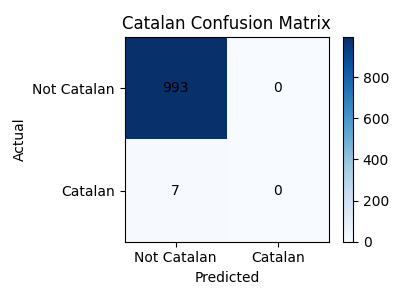
\includegraphics[width=0.45\textwidth]{plots/catalan_confusion.png}
    \caption{Catalan Confusion Matrix}
\end{figure}

\section{Conclusions}
This project demonstrates that a modular, NumPy-based neural network can successfully classify a wide variety of mathematical properties of numbers, with performance quantified by precision, recall, F1-score, and visualizations. The approach provides transparency, explainability, and immediate utility for mathematics and data science, and aligns with the goals of Zero Knowledge Proof by making number properties instantly accessible and verifiable.

\begin{thebibliography}{9}
\bibitem{zeroknowledgeproof}
Sánchez, J. M. (2024, May 22). What is zero Knowledge proof. Veridas. \url{https://veridas.com/en/what-is-zero-knowledge-proof/}
\bibitem{fibonnacisequence}
Sheldon, R. (2022, May 6). Fibonacci sequence. WhatIs; TechTarget. \url{https://www.techtarget.com/whatis/definition/Fibonacci-sequence}
\bibitem{neuralnetwork}
What is a neural network & how does it work? (n.d.). Google Cloud. Retrieved May 14, 2025, from \url{https://cloud.google.com/discover/what-is-a-neural-network?hl=en}
\end{thebibliography}

\end{multicols}
\end{document}